L'ultima fase dell'elaborato è verificare tramite simulazione che il modello funzioni e soddisfi le proprietà di safety e liveness richieste (si veda §\ref{Sec:prop}). Nell'ultimo paragrafo si discuterà anche della scalabilità del modello proposto.

In figura \ref{Fig:sims_30} sono mostrate le simulazioni effettuate osservando i segnali scambiati per 30 colpi di clock. Esamineremo prima il funzionamento delle code in tutti e due gli scenari e, poiché questa è l'unica differenza tra i due modelli, successivamente non tratteremo necessariamente entrambi i casi.

\begin{figure}
\centering
\vspace{-2cm}
\begin{subfigure}[t]{\textwidth}
	\centering
	\includegraphics[angle=-90, totalheight=\textwidth]{ep_30.eps}
	\vspace{-2.8cm}
	\caption{Equal Priority}
	\label{Fig:sim_ep_30}
\end{subfigure}
\begin{subfigure}[t]{\textwidth}
	\centering
	\includegraphics[angle=-90, totalheight=\textwidth]{fp_30.eps}
	\vspace{-2.8cm}
	\caption{Fixed Priority.}
	\label{Fig:sim_fp_30}
\end{subfigure}
\caption{Simulazioni di durata 30 colpi di clock eseguite con entrambi i modelli.}
\label{Fig:sims_30}
\end{figure}

%\clearpage

\subsection{Verifica della correttezza delle code di priorità}
Consideriamo prima il modello Equal Priority. In figura \ref{Fig:sim_ep_30} vengono mostrati sia le richieste dei processori che l'output del buffer FIFO. Il comportamento atteso è che, all'interno del buffer, una richiesta acquista tanta più priorità quanto più tempo è trascorso da quando è stata fatta. Questo è esattamente quello che succede: richieste che arrivano quando il buffer non è vuoto non vengono inoltrate al coordinatore fino a quando tutte le precedenti non sono state accolte, come è possibile notare dalla richiesta che il processore 1 effettua al tempo $t=9$. Se più richieste hanno priorità massima, ne viene scelta una in modo casuale.

Consideriamo ora il caso Fixed Priority, mostrato in figura \ref{Fig:sim_fp_30}. In questo scenario, un processore ha priorità tanto più alta quanto maggiore è il suo ID. Questo significa che, se ci sono richieste contemporanee da più processori, viene considerata solo quella del processore a priorità maggiore. Questo comportamento si può notare già al tempo $t=1$: tutti i processori hanno fatto richiesta, ma, come si evince dall'ultimo grafico, è la richiesta del processore 4 ad essere accolta (ed è soddisfatta dal bus 1).

\begin{figure}
\centering
\vspace{-2.8cm}
\includegraphics[angle=-90, totalheight=\textwidth]{ep_150.eps}
\vspace{-2.8cm}
\caption{Simulazioni di durata 150 colpi di clock eseguite con il modello Equal Priority.}
\label{Fig:sim_150}
\end{figure}

\subsection{Mutua esclusione nell'accesso ad un bus}
La proprietà di mutua esclusione può essere verificata già esaminando la macchina a stati del bus (figura \ref{Fig:bus_fsm}). Violare la mutua esclusione significa che, mentre il bus sta servendo un processore, accetta una richiesta proveniente da un processore diverso. Vediamo perché questo non è possibile.

Il segnale inviato allo switch dei processori viene impostato soltanto entrando nello stato \texttt{WaitingForProc} e viene resettato quando si smette di servire il processore (i.e., all'uscita dagli stati \texttt{Serving} o \texttt{ServingAndRelaying}). Questo significa che, mentre sta servendo, un bus può comunicare solo con il processore che ha fatto richiesta. D'altro canto, l'unico modo che il bus ha per uscire dagli stati Serving è ricevere un segnale di rilascio da parte del processore. Poiché il processore invia il segnale \texttt{release} soltanto quando smette di usare il bus (figura \ref{Fig:proc_fsm}), l'unico modo che il bus ha per iniziare la comunicazione con un altro processore è che il precedente effettui un rilascio. Questo garantisce la mutua esclusione nell'accesso ai bus.

La \textquotedblleft dimostrazione\textquotedblright{} teorica appena fornita è confermata dall'esito della simulazione: un bus garantisce l'accesso ad un processore soltanto se nessun altro processore possiede i diritti di accesso al bus, come è possibile notare dal secondo diagramma delle figure \ref{Fig:sims_30}.

\subsection{Assenza di livelock}
In linea di principio, con il modello adottato l'assenza di livelock non può essere garantita: è sempre possibile costruire un'esecuzione in cui più processori fanno richiesta e uno di essi non viene mai servito perché possiede priorità inferiore rispetto agli altri o perché tutti i bus sono già occupati. Tuttavia, come mostrano entrambe le figure \ref{Fig:sims_30} e \ref{Fig:sim_150}, nella pratica questa eventualità è rara: se i processori fanno richieste e rilasciano i bus ad intervalli di tempo casuali (e dello stesso ordine di grandezza), la probabilità che un processore debba attendere un intervallo di tempo infinito per accedere ad un bus è nulla.

\subsection{Assenza di deadlock}
Teoricamente, l'assenza di deadlock può essere verificata già dal diagramma del modello e dalle macchine a stati del coordinatore e dei bus, esaminando quali sono le condizioni per cui un automa non può più uscire da uno stato e controllando che esse non possano essere soddisfatte. Questo tipo di considerazioni sono state quelle che hanno guidato la modellazione degli automi, per cui il sistema è stato progettato prestando particolare attenzione a soddisfare questa proprietà. L'assenza di deadlock è stata poi verificata per via sperimentale: come si può vedere in figura \ref{Fig:sim_150}, in intervalli di tempo prossimi alla fine tutti i componenti funzionano ancora correttamente.

\subsection{Analisi di scalabilità}
Come si può vedere dalle figure \ref{Fig:proc_fsm}, \ref{Fig:coord_fsm} e \ref{Fig:bus_fsm}, nella definizione degli automi non vi è alcun parametro che faccia riferimento a quanti processori o bus siano presenti nel sistema. Inoltre, poiché all'interno di Scicos è possibile l'invio di messaggi broadcast e poiché un messaggio può essere ricevuto da un blocco e inoltrato nello stesso colpo di clock, l'incremento del numero di processori o di bus non comporta l'aumento del tempo necessario all'esecuzione dell'algoritmo di bus arbitration. Da questi punti di vista, quindi, il modello risulta facilmente scalabile.

La costruzione del modello, tuttavia, è stata effettuata con Scicos per via grafica. Questo significa che bisogna aggiungere manualmente ulteriori nodi processore o bus ed effettuare manualmente tutti i collegamenti necessari. Questa restrizione è piuttosto significativa ed è il motivo per cui, in ultima istanza, il modello risulta difficilmente scalabile.







